%%%%%%%%%%%%%% COPYRIGHT INFORMATION %%%%%%%%%%%%%%
% Template by
% Author: Sascha Frank 
% Nov. 2006
% University Freiburg 
% www.informatik.uni-freiburg.de/~frank/
% Distributed freely for non-commercial use

%%%%%%%%%%%%%%%%%%%%% PREAMBLE %%%%%%%%%%%%%%%%%%%%%
\documentclass{beamer}
\usepackage{beamerthemeshadow}
\usepackage{lmodern}
\usepackage{pifont}
\usepackage{color}

% include frame number on each frame
\setbeamertemplate{footline}{\quad \insertframenumber/\inserttotalframenumber}
\newcommand{\cmark}{\ding{51}} % check-mark
\newcommand{\xmark}{\ding{55}} % X-mark
\newcommand{\inv}{^{-1}}
\newcommand{\e}{\varepsilon}
\newcommand{\E}{\mathbb{E}}
\newcommand{\N}{\mathbb{N}}
\renewcommand{\P}{\mathbb{P}}
\newcommand{\R}{\mathbb{R}}
\newcommand{\Var}{\mathbb{V}}
\newcommand{\X}{\mathcal{X}}
\newcommand{\Y}{\mathcal{Y}}
\newcommand{\Z}{\mathcal{Z}}
\newcommand{\dist}{\operatorname{dist}}
\newcommand{\vi}{{\vec i}}
\renewcommand{\hat}{\widehat}

%%%%%%%%%%%%%%%%%%%%% DOCUMENT %%%%%%%%%%%%%%%%%%%%%
\begin{document}
\title{Regression}
\subtitle{Chapter 10 of \emph{Foundations of Machine Learning}, Pt. II}
\author[Singh]{Shashank Singh}
\date{April 20, 2015}
\institute{Carnegie Mellon University\\11-745 Spring '15}
\frame{\titlepage}

\frame{\frametitle{Outline}
\tableofcontents
}

\section{Regression Framework}
\frame{\frametitle{Problem Statement}
  \begin{itemize}
    \item size-$m$ sample $S = \{(x_1,y_1)\}_{i = 1}^m \in (\X \times \Y)^m$
          with
    \begin{itemize}
      \item $x_1,\cdots,x_m \sim D$ for some unknown distribution $D$ on $\X$
      \item $(y_1,\cdots,y_m) = (f(x_1),\cdots,f(x_m))$ for some unknown
            $f : \X \to \Y$
    \end{itemize}
    \item loss function $L : \Y \times \Y \to \R$
    \item want to find a hypothesis $h$ minimizing the risk
        \[R(h) = \E_{x \sim D}\left[ L(h(x), f(x)) \right].\]
  \end{itemize}
}

\section{More Algorithms}
\subsection{Support Vector Regression}
\frame{\frametitle{Fitting an $\e$-tube}
\begin{figure}[h]
\centering
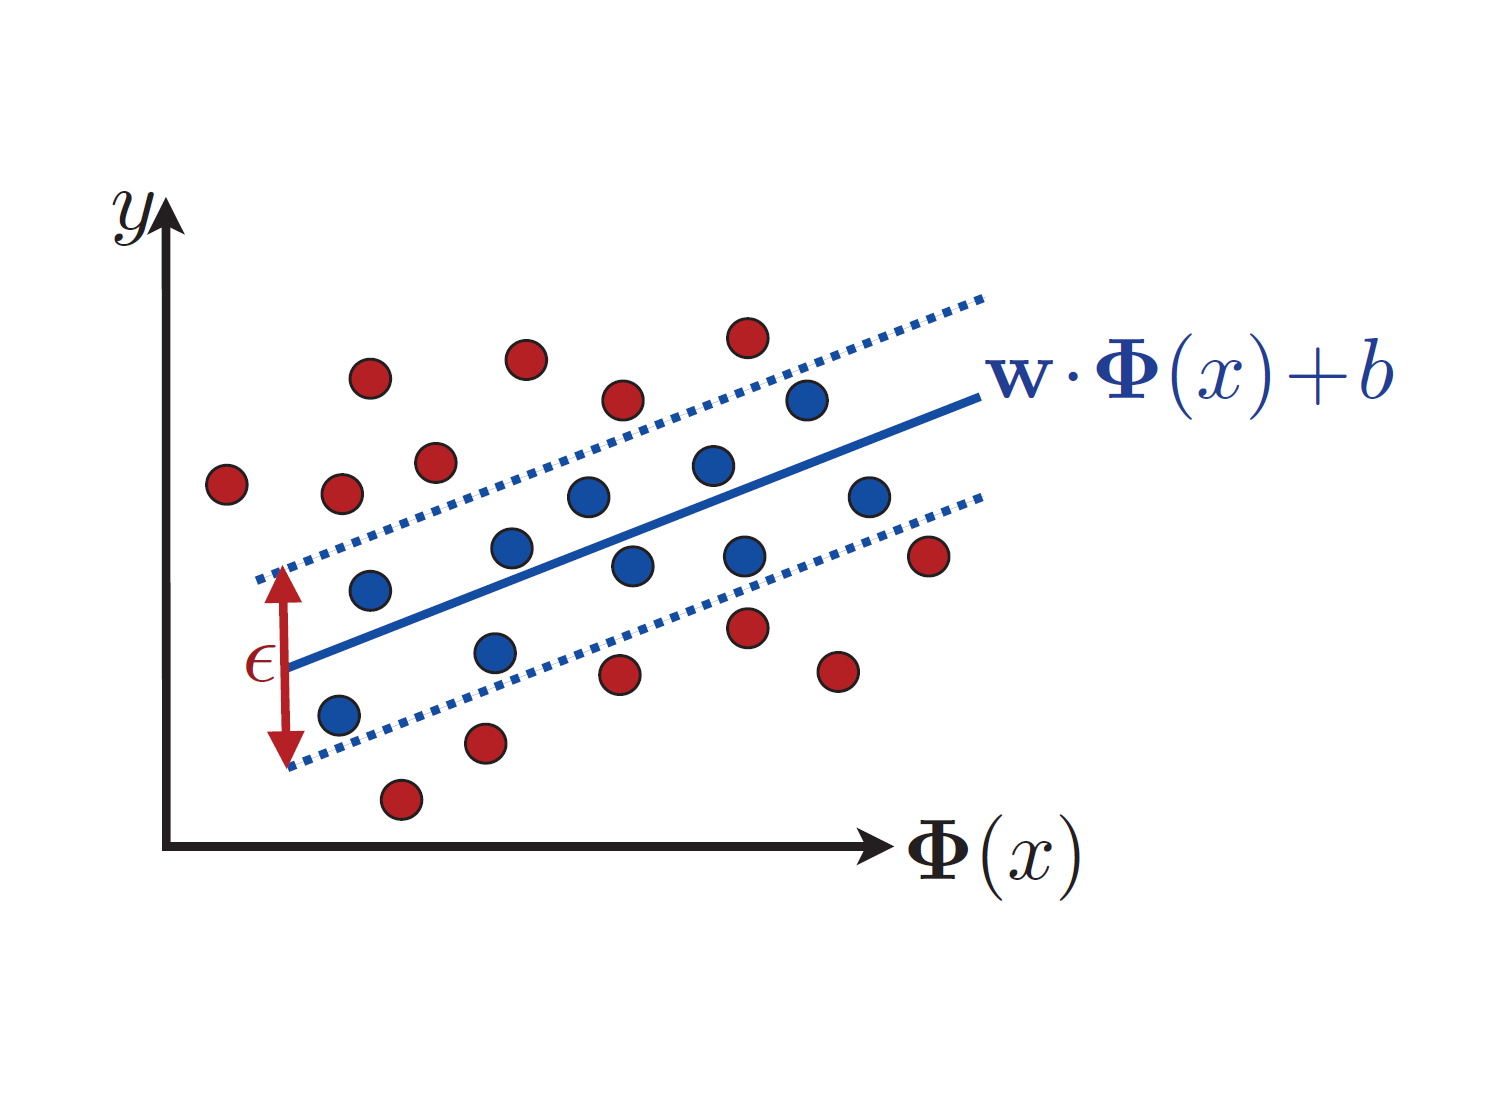
\includegraphics[width=0.75\textwidth,clip=true,trim=0mm 0mm 0mm 65mm]{SVR}
\vspace{-12mm}
\end{figure}
  \begin{itemize}
    \item Rather than fitting a line to the data, we fit an $\e$-tube
    \begin{itemize}
      \item Accordingly, we use the $\e$-insensitive loss
        \[L_\e(h(x), f(x)) = \max\{0,|h(x) - f(x)| - \e\}\]
    \end{itemize}
    \item This encourages a data-sparse solution, since points with
        $|\hat h(x_i) - y_i| \leq \e$ incur no loss
  \end{itemize}
}

\frame{\frametitle{Support Vector Regression}
  \begin{itemize}
    \item Apply feature map $\Phi : \X \to \R^{k}$ corresponding to kernel $K$
    \item Then fit a linear model:
        \[\hat f(x) = \hat w \cdot \Phi(x) + \hat b\]
    \item Thus, our empirical risk is
        \[\hat R(\hat w, \hat b)
            = \frac{1}{n} \sum_{i = 1}^n
                L_\e(\hat w \cdot \Phi(x_i) + \hat b, y_i)\]
    \item Finally, we add an $\ell_2$ regularization term on $w$ and parameter
          $C$, giving the optimization problem:
        \[\min_{w \in \R^k, b \in \R} \frac{1}{2}\|w\|_2^2
            + C\frac{1}{n} \sum_{i = 1}^n
                L_\e(\hat w \cdot \Phi(x_i) + \hat b, y_i)\]
  \end{itemize}
}

\frame{\frametitle{Deriving the Dual Problem}
  \begin{itemize}
    \item Add slack variables $\xi^-,\xi^+ \in \R^m$ which encode point loss:
      \begin{align*}
      \min_{w \in \R^k, b \in \R, \xi^-,\xi^+ \in \R_+^m}
                & \frac{1}{2}\|w\|_2^2
                  + \frac{C}{n} \sum_{i = 1}^n \xi^-_i + \xi^+_i    \\
      \mbox{subject to}
         \qquad & \hat w \cdot \Phi(x_i) + b \geq y_i - \e - \xi^-_i,   \\
                & \hat w \cdot \Phi(x_i) + b \leq y_i + \e + \xi^+_i
      \end{align*}
    \item $\xi^-_i$ and $\xi^+_i$ encode loss of under/overestimating $y_i$,
          resp.
    \item From here, we can derive the dual (as with SVMs):
      \begin{align*}
      \max_{\alpha,\alpha' \in \R^k}
              & -\e(\alpha' + \alpha)^T1_k + (\alpha' - \alpha)^Ty  \\
              & -\frac12 (\alpha' - \alpha)^T\mathbf{K}(\alpha' - \alpha) \\
      \mbox{subject to}
         \qquad & 0 \leq \alpha_i, \alpha'_i \leq C,  \\
                & (\alpha' - \alpha)^T 1_k = 0
      \end{align*}
  \end{itemize}
}

\frame{\frametitle{Computing SVR Solutions}
  \begin{itemize}
    \item Both the primal and the dual are quadratic programs
      \begin{itemize}
        \item can be solved via standard algorithms
      \end{itemize}
    \item Can recover the hypothesis $h$ from $(\alpha,\alpha')$ via
        \[h(x) = b + \sum_{i = 1}^m (\alpha' - \alpha)K(x_i,x),
                                                    \quad \forall x \in \X\]
        where, for any $x_j$ with $\alpha_j \in (0,C)$ or $\alpha'_j \in (0,C)$
        \[b = -\sum_{i = 1}^m (\alpha' - \alpha)K(x_i,x_j) + y_j \pm \e\]
    \item Thus, we can solve either the primal or the dual
    \item By complementarity, only points outside $\e$-tube are support vectors
    \item $\e$ provides trade-off between sparsity and accuracy
  \end{itemize}
}

\frame{\frametitle{SVR Generalization Bounds}
{\bf Theorem 10.8:}
\begin{itemize}
\item $K : \X \times \X \to \R$ PDS kernel with feature map
$\Phi : \X \to \mathbb{H}$
\item $H := \{x \mapsto w \cdot \Phi(x) : \|w\|_{\mathbb{H}} \leq \Lambda\}$
\item
\[r := \sup\left\{\sqrt{K(x,x)}, \frac{|f(x)|}{\Lambda} : x \in \X\right\}\]
\end{itemize}
Then, w.p. $\geq 1 - \delta$,
\[R_\e(h) \leq \hat R(h) + \frac{2r\Lambda}{\sqrt m}
                    \left( 1 + \sqrt{\frac{\log(1/\delta)}{2}} \right)\]
and
\[R_\e(h) \leq \hat R(h) + \frac{2r\Lambda}{\sqrt m}
                \left( \sqrt{\frac{Tr[K]}{mr^2}}
                                + 3\sqrt{\frac{\log(1/\delta)}{2}} \right).\]
\begin{itemize}
\item The theorem follows from results proven last time.
\end{itemize}
}

\frame{\frametitle{Strengths and Weaknesses of SVR}
  \begin{itemize}
    \item Strengths:
      \begin{itemize}
        \item Strong theoretical guarantees (gen. error and stability)
        \item Data-sparsity (assuming $\e$-insensitive loss)
        \item Non-linearity and expert knowledge integration via PDS kernels
        \item Regularization
      \end{itemize}
    \item Weaknesses:
      \begin{itemize}
        \item Two parameters to select ($C$ and $\e$; heuristics exist)
        \item Computationally expensive for large training sets
          \begin{itemize}
          \item Can make kernel evaluation more efficient via low-rank
                approximations
          \end{itemize}
      \end{itemize}
  \end{itemize}
}

\subsection{Lasso}

\frame{\frametitle{Lasso}
  \begin{itemize}
    \item Unlike KRR and SVR, Lasso is not kernelizable, so let
      \begin{itemize}
      \item $\X \subseteq \R^N$
      \item $H = \{x \mapsto w \cdot x + b : w \in \R^N, b \in \R\}$
      \end{itemize}
    \item We optimize the following:
        \[\min_{w \in \R^N, b \in \R} \lambda\|w\|_1
                                + \sum_{i = 1}^N (w \cdot x_i + b - y_i)^2\]
    \item This induces sparsity in $w$
\end{itemize}
}

\frame{\frametitle{Lasso}
  \begin{itemize}
    \item For some $\Lambda_1 > 0$, this optimization problem is equivalent to
        \[\min_{w \in \R^N, b \in \R} \sum_{i = 1}^N (w \cdot x_i + b - y_i)^2
        \quad \mbox{ subject to } \quad \|w\|_1 \leq \Lambda_1\]
\end{itemize}
\begin{figure}[h]
\centering
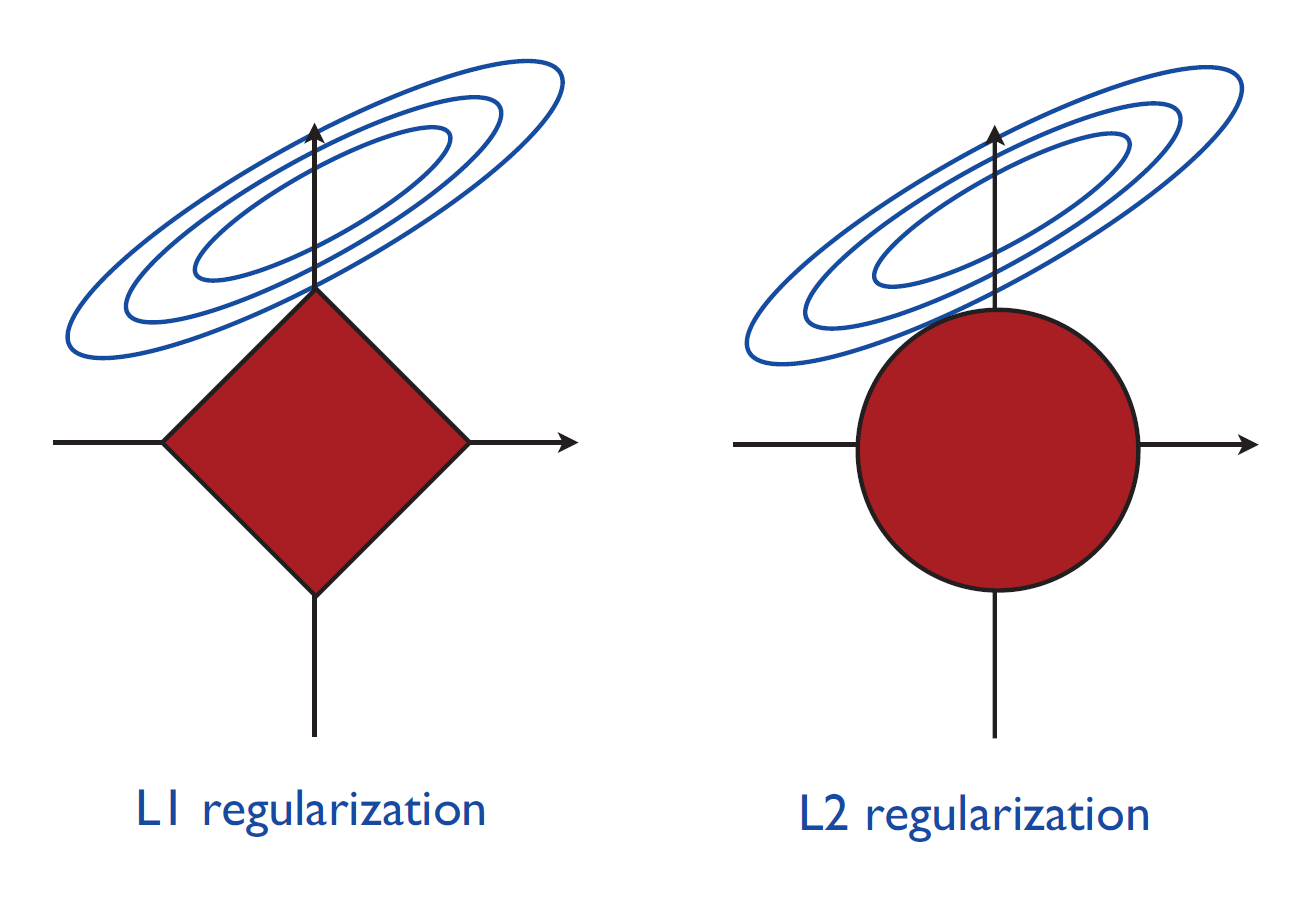
\includegraphics[width=0.75\textwidth,clip=true,trim=0 0 0 20mm]{lasso}
\end{figure}
}

\frame{\frametitle{Rademacher complexity of lasso (with bounded $L_1$ norm)}
{\bf Theorem 10.10:}
\begin{itemize}
\item $\X \subseteq \R^N$
\item $r = \max_{i \in [1,m]} \|x_i\|_\infty$
\item $H := \{x \mapsto w \cdot x : \|w\|_1 \leq \Lambda_1\}$
\end{itemize}
Then,
\[\hat {\mathfrak R}_S(H)
    \leq \sqrt{\frac{2r_\infty^2\Lambda_1^2\log(2N)}{m}}\]
\begin{itemize}
\item Note the logarithmic dependence on dimension $N$
\item Deterministic bound on empirical Rademacher complexity of a given sample
\end{itemize}
}

\frame{\frametitle{Proof of Generalization Bound}
First recall two facts:
\begin{enumerate}
\item Dual norms: For $p,q \in [1,\infty]$, if $\frac{1}{p} + \frac{1}{q} = 1$,
      then $\forall x \in \R^n$,
    \[\|x\|_p
        = \left( \sum_{i = 1}^n x_i^p \right)^{1/p}
        = \sup_{\|y\|_q \leq 1} y \cdot x.\]
\item Massart's Lemma: For $A \subseteq \R^n$ finite,
$r := \max_{x \in A} \|x\|_2$,
\[\E_\sigma\left[ \frac{1}{m} \sup_{x \in A} \sum_{i = 1}^m \sigma_ix_i \right]
    \leq \frac{r\sqrt{2 \log |A|}}{m}.\]
\end{enumerate}
}

\frame{\frametitle{Proof of Generalization Bound}
Since $\|\cdot\|_1$ and $\|\cdot\|_\infty$ are dual norms,
\begin{align*}
\hat {\mathfrak R}_S(H)
 &  = \frac{1}{m} \E_\sigma \left[
        \sup_{\|w\|_1 \leq \Lambda_1} w \cdot \sum_{i = 1}^m \sigma_i x_i
      \right]   \\
 &  = \frac{\Lambda_1}{m} \E_\sigma
        \left[ \left\| \sum_{i = 1}^m \sigma_i x_i \right\|_\infty \right]
    = \frac{\Lambda_1}{m} \E_\sigma
        \left[ \sup_{z \in A} \sum_{i = 1}^m \sigma_i z_i \right]
\end{align*}
for $A = \{s(x_{1,j},\cdots,x_{m,j})^T : j \in [1,N], s \in \{-1,1\}\}$.

For $z \in A$, $\|z\|_2 \leq \sqrt{mr_\infty^2} = r_\infty\sqrt m$. Thus, by
Massart's Lemma, since $|A| \leq 2N$,
\[\hat {\mathfrak R}_S(H)
    \leq \Lambda_1r_\infty\sqrt{m}\sqrt{\frac{2\log(2N)}{m}}
    \leq \sqrt{\frac{2r_\infty^2\Lambda_1^2\log(2N)}{m}}.\]
}

\frame{\frametitle{Rademacher complexity of lasso (with bounded $L_1$ norm)}
{\bf Theorem 10.11:}
\begin{itemize}
\item $\X \subseteq \R^N$
\item $r = \sup_{x \in \X} \|x\|_\infty$
\item $H := \{x \mapsto w \cdot x : \|w\|_1 \leq \Lambda_1\}$
\end{itemize}
Then, w.p. $\geq 1 - \delta$,
\[R(h)
    \leq \hat R(h) + \frac{8r_\infty^2\Lambda_1^2}{\sqrt{m}}
    \left( \sqrt{2\log(2N)} + \frac12\sqrt{\frac{\log(1/\delta)}{2}} \right).\]
\begin{itemize}
\item High prob. gen. bound for bounded domain (unlike 10.10)
\item Follows from previous results, including Theorem 10.10
\end{itemize}
}

\frame{\frametitle{Strengths and Weaknesses of Lasso}
  \begin{itemize}
    \item Strengths:
      \begin{itemize}
        \item Strong theoretical guarantees (gen. error and stability)
        \item Fast algorithms (Lars) for computing entire \emph{regularization
              path}
        \item Efficient online version
        \item Feature-sparsity
      \end{itemize}
    \item Weaknesses:
      \begin{itemize}
        \item Not kernelizable, and hence only linear
              \begin{itemize}
                \item Can use empirical kernel maps
              \end{itemize}
        \item No closed form solution
      \end{itemize}
  \end{itemize}
}

\frame{\frametitle{Group Norm Regression Algorithms}
  \begin{itemize}
    \item If the feature space naturally partitions into subsets, we can
          encourage a sparse solution that selects groups of features
    \item If $w = (w_1,\cdots,w_k) \in \R^N$, where each $w_i \in \R^{N_i}$,
          then the $L_{2,1}$ norm of $w$ is
            \[\|w\|_{2,1} = \sum_{i = 1}^k \|w_i\|_2.\]
  \end{itemize}
}

\section{Online Algorithms}
\subsection{Widrow-Hoff Algorithm}
\frame{\frametitle{Widrow-Hoff Algorithm}
\begin{figure}[h]
\centering
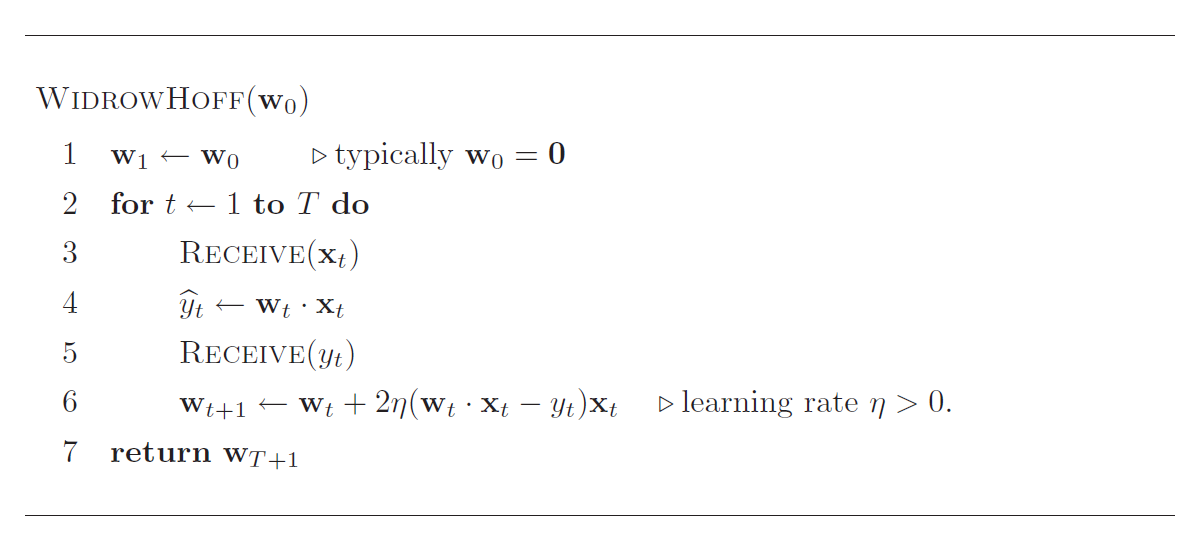
\includegraphics[width=\textwidth]{widrowhoff}
\vspace{-6mm}
\end{figure}
  \begin{itemize}
    \item Applies online gradient descent to least squares objective
    \item Can do the same with ridge regression and lasso
  \end{itemize}
}
\subsection{Online Dual SVR}
\frame{\frametitle{Online Dual SVR}
\begin{figure}[h]
\centering
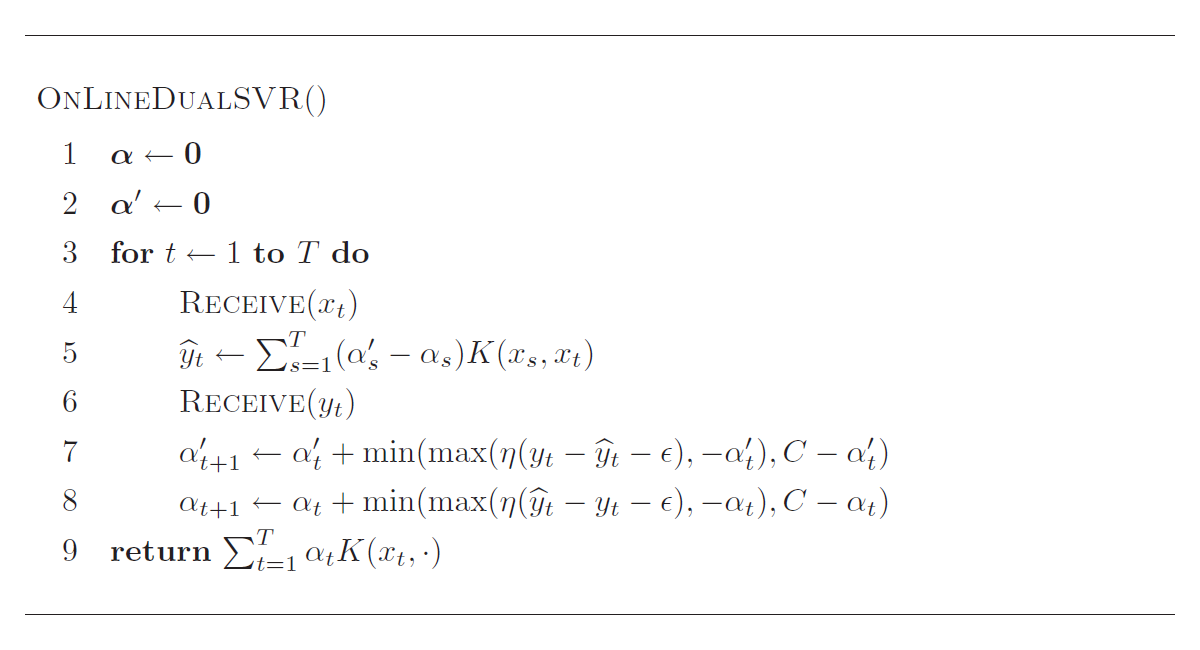
\includegraphics[width=\textwidth]{onlineSVR}
\vspace{-6mm}
\end{figure}
  \begin{itemize}
    \item Applies online gradient descent to dual SVR objective
  \end{itemize}
}

\section{Nonparametric Algorithms}
\frame{\frametitle{Nonparametric Regression}
  \begin{itemize}
    \item Want to fit
        \[y = f(x) + \e,\]
          where $f$ is smooth, but need not be linear
    \item Can still use penalized risk minimization approaches (e.g., splines)
    \item Here, we'll mention a different method
  \end{itemize}
}

\subsection{Local Polynomial Regression}
\frame{\frametitle{Local Polynomial Regression}
  \begin{itemize}
    \item Let $w_i(x)$ denote the weight of the data point $(x_i,y_i)$ on the
prediction at $x$.
\begin{itemize}
\item Usually, $w_i(x)$ is based on a smoothing kernel, e.g.,
\[w_i(x)
    = \frac{1}{\sqrt{2\pi h^2}}\exp\left( -\frac{(X_i - x)^2}{2h^2} \right),\]
where $h > 0$ is a bandwidth parameter
\end{itemize}
    \item Let $P_x(X;a)$ denote the order $p$ polynomial with coefficients
$(a_1,\cdots,a_p)$,
evaluated at $X - x$:
        \[P_x(X;a) = \sum_{j = 1}^p \frac{a_p}{p!}(X - x)^p\]
\end{itemize}
}

\frame{\frametitle{Local Polynomial Regression}
  \begin{itemize}
    \item For weights $w_i(x)$ (e.g., from a smoothing kernel), minimize
        \[\min_{a \in \R^p} \sum_{n = 1}^n w_i(x)(Y_i - P_x(X_i;a))^2\]
    \item If
\vspace{-5mm}
        \[X_x = \begin{bmatrix}
            1 & X_1 - x & \cdots & \frac{(X_1 - x)^p}{p!}   \\
            \vdots & \vdots & \ddots & \vdots   \\
            1 & X_n - x & \cdots & \frac{(X_n - x)^p}{p!}
        \end{bmatrix},
        W = \text{diag}(w_1(x),\cdots,w_n(x)),\]
        then
        \[\sum_{n = 1}^n w_i(x)(Y_i - P_x(X_i;a))^2
                                                = (Y - X_xa)^TW_x(Y - X_xa),\]
        and so $\hat a(x) = (X_x^T W_x X_x)\inv X_x^T W_x Y$
        (closed form solution)
  \end{itemize}
}

\frame{\frametitle{Nonparametric Theory}
  \begin{itemize}
    \item Rademacher complexity is usually infinite for nonparametric
          hypothesis classes
    \item Rather than generalization bounds, results are usually bounds on bias
          and variance of $\hat f$, either at a point or integrated
    \item Bias bounds depend crucially on smoothness assumptions on true $f$,
          e.g.
          \[L = \int_\R (f^{(\beta)}(x))^2 \, dx < \infty,\]
          where $\beta \in \mathbb{N}$ and $f^{(\beta)}$ the $\beta$-order
          derivative of $f$
  \end{itemize}
}

\end{document}
